\documentclass[12pt]{article}

\usepackage[utf8x]{inputenc}
\usepackage{hyperref}
\usepackage{minted}
\usepackage{graphicx}

\title{Inteligență Aritificială \\ Tema 1: \emph{Biscuitele}}
\author{Tudor Berariu \\ \emph{tudor.berariu@gmail.com}}

\begin{document}
\maketitle

\section{Descrierea jocului}
\label{sec:desc}

Jocul \emph{Dots and Boxes} se desfășoară pe o matrice de dimensiune
$height \times width$. Importante sunt cele $(height+1) \times
(width+1)$ puncte de intersecție. În timpul jocului, pe rând, fiecare
dintre cei doi jucători unește două puncte vecine cu o linie
orizontală sau verticală. Scopul este acela de a închide cât mai multe
celule prin unirea punctelor. Fiecare jucător primește un punct pentru
fiecare celulă pe care o închide (toți cei patru pereți care
delimitează celula au fost adăugați). La finalul jocului câștigă acel
jucător care a strâns mai multe puncte.

\begin{figure}[h]
  \centering
  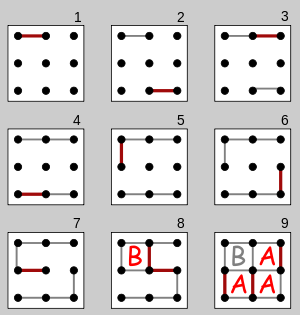
\includegraphics[width=.3\textwidth]{dots.png}
  \caption{Sursa imaginii: \url{https://en.wikipedia.org/wiki/Dots_and_Boxes}}
\end{figure}

Jucătorii \emph{mută} alternativ, dar un jucător care reușește în urma
unei mutări să închidă o celulă mai primește dreptul la încă o mutare.

\section{Cerințe și notare}
\label{sec:tasks}

Implementați algoritmul MiniMax pentru jocul \emph{Dots and
  Boxes}. Algoritmul trebuie completat de tehnica $\alpha-\beta$
pruning. Găsiți o euristică cât mai bună astfel încât să bateți cei
doi jucători implementați deja.

Există o limită de timp de o secundă pe mutare. La depășirea ei, jocul
respectiv se consideră pierdut.

Tema va fi testată pe matrice de dimensiuni $7\times 7$, $11 \times
11$ și $15 \times 15$.

Se vor acorda \textbf{5 puncte} pentru implementarea algoritmului
MiniMax cu $\alpha-\beta$ pruning.

Se vor acorda \textbf{5 puncte} pentru găsirea unei euristici destul
de bune încât să bată jucătorii pe care îi găsiți în arhiva temei.

Se vor acorda până la \textbf{2 puncte bonus} pentru cele mai bune
50\% dintre teme. Toate soluțiile trimise vor fi confruntate, se va
face un clasament general, iar prima jumătate din acel clasament va
primi de la 2 la 0.5 puncte (descrescător în ordinea
punctajului). Clasamentul va fi făcut întâi după numărul de jocuri
câștigate și apoi după numărul total de puncte adunate.

\section{Arhiva temei}
\label{sec:arhiva}

Arhiva temei conține un script \texttt{game\_server.py} care confruntă
toți jucătorii din directorul \texttt{players}. Fiecare jucător este
implementat într-un fișier separat în care se găsește o clasă cu
același nume. În arhivă găsiți două implementări simple de jucători.

Pentru a vă testa soluția, implementați o soluție, puneți fișierul în
directorul \texttt{players} și rulați \texttt{make clean} și
\texttt{make}.

Dacă aveți \texttt{pdflatex} și desktop Gnome, puteți rula comanda
\texttt{make pdf} și se va deschide un pdf cu clasamentul jucătorilor.

\section{Trimiterea temei}
\label{sec:archive}

Arhiva temei va conține un fișier \texttt{PDF} cu descrierea soluției
folosite în temă și un \emph{singur} fișier \texttt{Python} cu
implementarea soluției. Fișierele vor avea un nume construit astfel:
\texttt{NumePrenumeAAAALLZZ.ext} din numele complet și data
nașterii. Renunțați, desigur la diacritice și la linii. \texttt{ext}
va fi \texttt{pdf} sau \texttt{py}.

În fișierul \texttt{Python} se va găsi o clasă cu același nume în care
vor fi cel puțin următoarele două metode: \texttt{\_\_init\_\_} și \texttt{move}.

\begin{minted}{python}
  class LionelMessi19870624:
    def __init__(self):
      self.name = "Lionel Messi"

    def move(self, board, score):
      return (0,0)
\end{minted}

Metoda \texttt{\_\_init\_\_} va inițializa un câmp \texttt{name} cu un șir
de caractere ce conține numele complet.

Metoda \texttt{move} primește două argumente: \texttt{board} și \texttt{score}:
\begin{itemize}
\item \texttt{board} este o listă cu $height * 2 + 1$ liste. Cele de
  pe pozițiile pare ($0, 2, \ldots, height * 2$) corespund liniilor
  orizontale și au lugime $width$. Listele de pe pozițiile impare
  corespund liniilor verticale și au lungime $width + 1$.
\item \texttt{score} reprezintă un tuplu cu scorul curent: punctajul
  propriu, punctajul adversarului.
\end{itemize}
Funcția \texttt{move} întoarce un tuplu \texttt{(linie, coloana)} din
\texttt{board} ce corespunde liniei ce se dorește trasată.

\paragraph{Exemplu de matrice}

Pentru matricea următoare:
\begin{verbatim}
*-* * *
| |   |
* * *-*
  | |  
* * * *
|      
*-*-*-*
\end{verbatim}
parametrul \texttt{board} va fi:
\begin{verbatim}
[[1, 0, 0],
 [1, 1, 0, 1],
 [0, 0, 1],
 [0, 1, 1, 0],
 [0, 0, 0],
 [1, 0, 0, 0],
 [1, 1, 1]]
\end{verbatim}

În arhiva pe care o încărcați pe \url{curs.cs} puneți direct cele două
fișiere (nu un director).

\end{document}
